%% ****** Start of file rsitemplate.tex ****** %
%%
%%   This file has been edited from the original source file.
%%	 The original file is part of the revtex4-1 package indicated below.
%%   Version 4.1 of 9 October 2009.
%%
%
% This is a template for producing documents for use with 
% the REVTEX 4.1 document class and the RSI substyle.
% 
% Copy this file to another name and then work on that file.
% That way, you always have this original template file to use.
\documentclass[aip,rsi,reprint]{revtex4-1} % for checking your page length
%\documentclass[aip,rsi,reprint,graphicx,draft]{revtex4-1} % for checking your page length
%\\documentclass[aip,rsi,preprint,graphicx]{revtex4-1} % for review purposes

\usepackage{siunitx}
\DeclareSIUnit{\sqrthz}{\ensuremath{\sqrt{\text{\hertz}}}}

\usepackage{amsmath}
\usepackage{amsfonts}

\usepackage{graphicx}
\usepackage{dcolumn}
\usepackage{multirow}
%\usepackage{caption}
%\usepackage{subcaption}

%% Work with illustrator *.ai files...
\DeclareGraphicsRule{.ai}{pdf}{.ai}{}


%% useful macros
\newcommand{\epar}{~||~} % add impedances in parallel


\begin{document}

% Use the \preprint command to place your local institutional report number 
% on the title page in preprint mode.
% Multiple \preprint commands are allowed.
%\preprint{}

\title{An ultra-low noise, high-voltage piezo driver}

% repeat the \author .. \affiliation  etc. as needed
% \email, \thanks, \homepage, \altaffiliation all apply to the current author.
% Explanatory text should go in the []'s, 
% actual e-mail address or url should go in the {}'s for \email and \homepage.
% Please use the appropriate macro for the type of information

% \affiliation command applies to all authors since the last \affiliation command. 
% The \affiliation command should follow the other information.

\author{N.C. Pisenti}
\email[]{npisenti@umd.edu}
\author{B.J. Reschovsky}
\author{D.S. Barker}
\author{A. Restelli}
\author{G.K. Campbell}
%\homepage[]{Your web page}
%\thanks{}
%\altaffiliation{}
\affiliation{Joint Quantum Institute, University of Maryland and National Institute of Standards and Technology}

% Collaboration name, if desired (requires use of superscriptaddress option in \documentclass). 
% \noaffiliation is required (may also be used with the \author command).
%\collaboration{}
%\noaffiliation

\date{\today}

\begin{abstract}
We present an ultra-low noise, high voltage driver suited for use with piezoelectric actuators and other low-current applications.
The architecture leverages a commercially available, small-form-factor integrated circuit (IC) for generating high voltage outputs.
The IC uses a flyback configuration switching regulator to generate up to 250V in our design (but up to 1kV or more with small modification), and a high slew-rate op-amp capacitively coupled to the output compensates for the switching noise.
A low-voltage (\SI{\pm 10}{\volt}), high bandwidth modulation input is capable of summing small voltage corrections onto the output, making the driver well suited for use in closed-loop feedback applications.
\end{abstract}

\pacs{}% insert suggested PACS numbers in braces on next line

\maketitle %\maketitle must follow title, authors, abstract and \pacs

% Body of paper goes here. Use proper sectioning commands. 
% References should be done using the \cite and \label commands
\section{Introduction}
\label{Sec:Introduction}

Many instrumentation applications in the modern laboratory require agile, low-noise voltage sources capable of supplying hundreds of volts or more.
For example, piezo-actuated mirrors and diffraction gratings play an important role in many atomic physics experiments (used, e.g., in scanning Fabry-Per{\`o}t cavities and extended-cavity diode lasers).
Avalanche photodiodes require a low-noise reverse bias of a few hundred volts or more (cite paper Alessandro/Prasoon are using?).
Other applications...? biophysics? medical devices?

Often, these applications are operated in a closed feedback loop, where small voltage changes on top of a large DC voltage are necessary to stabilize the output of a particular system.
For example, extended-cavity diode lasers adjust their lasing frequency by changing the angle of a diffraction grating that supplies optical feedback to the diode.
To stabilize this frequency, a servo controller measures deviations from the desired value and adjusts the voltage controlling the grating angle to correct for any difference.
Because the servo electronics operate at low voltage, a secondary high-voltage (HV) amplifier is required to drive the piezoelectric actuator.
This HV gain stage typically accepts an external ``modulation input'', $V_{\text{mod}}$, and produces an amplified voltage $V_{\text{out}}$ according to
\begin{align}
V_{\text{out}} = G_p V_{\text{mod}} + V_0
\end{align}
where $G_p$ is the amplifier gain and $V_0$ is an optional DC offset.
Typically, {$G_p\approx \num{10} - \num{20}$} or more such that reasonable voltages $V_{\text{mod}}$ can span the entire output range $V_{\text{out}}$.

It is often the case, however, that in closed-loop feedback applications we do not need and often do not want the modulation control to have a high gain.
Because the closed loop gain $G \equiv G_s G_p$ cannot be increased without limit, $G_p \gg 1$ means the servo gain $G_s$ must be proportionally smaller to keep the lock stable.
In locked configuration, any noise introduced by the servo is suppressed by $1/|G_s|$ in the large gain limit.
If $G_s$ is limited to achieve a stable lock, it is no longer effective at servoing its own noise.

To avoid this problem, we desire a high voltage amplifier which separates the ``setpoint'' gain, $G_{\text{dc}}$, from the modulation gain, $G_{\text{mod}}$. That is,
\begin{align}
  V_{\text{out}} &= G_{\text{dc}} V_{\text{dc}} + G_{\text{mod}} V_{\text{mod}}\, \text{,}
  \label{Eq:PiezoTransfer}
\end{align}
where now we can make $G_{\text{mod}} \approx 1$.

Traditionally, laboratory electronics capable of supplying high voltages fall under one of two architectural umbrellas: switching converters, and ``linear'' amplifiers.
DC-DC converters are efficient and can work at very high voltages, but suffer from switching noise and limited control bandwidths.
Linear-type devices are typically constructed from a high-voltage operational amplifier (op-amp), powered either from a high voltage linear regulator or more typically from a secondary switching converter.
While the op-amp provides \SI{100}{\decibel} or more of power-supply noise rejection, a high-voltage op-amp requires substantially more power than an equivalent switching circuit.
In either case, the output voltage  $V_{\text{out}}$ is typically given by
\begin{align}
  V_{\text{out}} &= G_p(V_{\text{DC}} + V_{\text{mod}})\, \text{,}
\end{align}
where $G_p$ is the piezo amplifier gain, $V_{\text{DC}}$ is a DC setpoint, and $V_{\text{mod}}$ is a modulation input used for closed-loop control.

\section{Circuit Design}
\label{Sec:Circuit}

The design is based on the newly-available Texas Instruments DRV2700 piezo driver.
\footnote{The identification of commercial products is for information only and does not imply recommendation or endorsement by the National Institute of Standards and Technology.}
This single-chip integrated circuit (IC) can be operated as a boost converter to drive an on-chip differential amplifier up to \SI{100}{\volt}, or as a flyback converter up to \SI{1}{\kilo\volt}.
In flyback configuration, the internal-boost switch of the DRV2700 drives a step-up transformer.
When the switch closes, current begins to flow through the primary coil of the transformer and induces a corresponding voltage across the secondary coil.
In this state, the output diode is reverse-biased, and the capacitor ($\text{C}_{\text{HV}}$ in Fig.~\ref{Fig:PiezoCircuit}) holds its charge.
When the switch opens, the voltage across the secondary coil is inverted, putting the diode into conduction and charging the capacitor.
%One key benefit of this topology is the galvanically isolated output.
%By sensing the output voltage across a resistive divider, we feed back to the floating ground from the flyback converter to remove switching noise and stabilize the high voltage output; see Fig.~\ref{Fig:PiezoCircuit}.

\begin{figure*}[t]
\includegraphics[width=\textwidth]{fig/DRV2700.ai}
\caption{Schematic of the high voltage stabilization.
The voltage HV is generated using a Texas Instruments DRV2700 high voltage driver in flyback configuration (see Fig.~\ref{Fig:DRV2700}).
A fast, very high slew-rate op-amp senses the output voltage across $R_1$ and $R_2$, and servos it by modulating the node at ``HV floating gnd''.
The $V_{\text{DC}}$ gain is set by $\left(1+R_1/R_2\right)$, while the modulation gain is set by $-R_{\text{mod}}/R_{\text{fb}}$.
The capacitor linking the floating ground node to the output allows the op-amp to remove residual switching noise and stabilize the DC output according to the transfer function given in Eq.~(\ref{Eq:PiezoTransfer}). \label{Fig:PiezoCircuit}}
\end{figure*}

In isolation, the DRV2700 is not suited for low-noise laboratory instrumentation. 
The output ripple, even after heavy filtering, can be as high as a few volts, and standard filtering techniques to reduce this noise simultaneously reduces the modulation bandwidth of the flyback regulator.
Even if this were not the case, it remains unlikely that the RMS noise could be brought below $\SI{1}{\milli\volt}$, which is the operating regime we require for certain low-noise applications in the laboratory.
Despite this drawback, the flyback converter requires very little current to operate and leverages a compact IC to generate very high voltages, making it versatile and easy to deploy in the lab.

The motivation behind our hybrid architecture is twofold.
First, to make a switching converter useful for low-noise laboratory instrumentation, we need a way to remove the output ripple and residual switching noise.
Second, we want to take advantage of low-noise op-amps that only work up to tens of volts to provide a unity gain (DC-coupled) feedback path to the high voltage output.
The architecture shown in Fig.~\ref{Fig:PiezoCircuit} does just this; a low-noise, high-slew rate op-amp ($\mathbf{U2}$) adjusts the floating ground node of the transformer output to cancel switching noise and sum in an offset given by $V_{\text{mod}}$, while the flyback regulator works close to DC to impose the high voltage across the HV - floating ground output.
We now explain the operation of each sub-block, and draw attention to important design details.

\subsection{DRV2700 flyback regulator}
\label{Sec:DRV2700}

We based the flyback regulator design off the suggested schematic in the DRV2700 datasheet and evaluation module application note.
At a basic level, the DRV2700 flyback circuit requires a transformer (ATB3225; 1:10 step-up winding, \SI{7}{\micro\henry} inductance, rated for \SI{0.6}{\ampere}) connected to an output diode and capacitor, and a ``sense'' voltage supplied to the feedback (FB) node of the IC.
Internally, the DRV2700 boost controller tries to drive the FB node to \SI{1.3}{\volt}.
The op-amp U1 senses the voltage at node \textit{HV} and \textit{GND}${}_\text{HV}$, and adjusts its output such that
\begin{align}
\label{Eq:U1Output}
\text{HV} &= G\cdot V_{\text{dc}} + \text{GND}_{\text{HV}}\,,
\end{align}
where the gain $G$ is set by the resistor ratio $R_3/R_4 \equiv R_5/R_6$.
The capacitors $C_3$ and $C_4$ are chosen such that $C_3 = \SI{22}{\pico\farad}$ and 
\begin{align}
\frac{C_4}{C_3} &= \frac{R_3}{R_4~||~R_5}\,,
\end{align}
as suggested by the datasheet.
This pseudo-differential configuration ensures that, in the equilibrium given by Eq.~(\ref{Eq:U1Output}), the output of U1 is driven to \SI{0}{\volt}; the resistive divider $R_9$ and $R_{10}$ is then chosen such that $R_9/(R_9~||~R_{10}) = \SI{1.3}{\volt}/\SI{5}{\volt} \approx \num{0.26}$.



Notes here about expected, measured bandwidth??

The DRV2700 IC, combined with the the feedback provided by U1, regulates the voltage $(\text{HV}-\text{GND}_{\text{HV}}) = G\cdot V_{\text{dc}}$.
Careful attention was paid to the layout ...

\subsection{Low-noise stabilization}
\label{Sec:LowNoiseStabilization}

The low-noise stabilization circuitry was added to remove output ripple and residual switching noise, however it serves a dual purpose as a low-gain, high-bandwidth modulation path to the high-voltage output.
It uses a very high slew-rate (\SI{4100}{\volt\per\micro\second}) op-amp, the LM7171, connected to the filtered ground node of the flyback converter.
At high frequencies, the output of this op-amp appears directly at the HV node through the capacitor $C_{\text{out}}$.
Below the corner set by $C_{\text{out}}$, the output of U2 adjusts the floating ground reference of the flyback converter.

After the passive filter ladder connecting the DRV2700 flyback converter the output,
%At high frequencies, this modulation appears directly at the HV node through the capacitors.
%At quasi-DC frequencies, the flyback regulator adjusts the HV node to keep 

The choice of component for resistors $R_1$ and $R_2$ is crucial for the low-noise performance of the system. (cite LIGO paper)

For a detailed noise analysis, see Sec.~\ref{Sec:NoiseAnalysis}.

\subsection{Digital control and auxiliary design features}
\label{Sec:DigControlAuxDesign}

\subsection{Noise Analysis}
\label{Sec:NoiseAnalysis}

\begin{figure}[t]
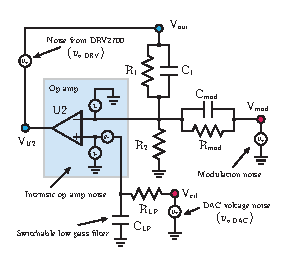
\includegraphics[width=\columnwidth]{fig/NoiseModel.ai}
\caption{Noise model. \label{Fig:NoiseModel}}
\end{figure}

We analyze the noise performance of the circuit according to the model shown in Figure~\ref{Fig:NoiseModel}, where noise spectral densities are calculated at the node HV.
Here, we consider contributions from the intrinsic op-amp noise, the DAC (injected at the node $V_{\text{DC}}$), Johnson-Nyquist noise of the passive components, and any additional noise injected at the modulation input node $V_{\text{mod}}$.
We also discuss, given our choice of op-amp, the noise rejection ratio from the DRV2700 flyback regulator.

First, the noise gain ($NG$) for this amplifier configuration is given by
\begin{align}
\label{Eq:NG}
%NG(s) &= 1 + \frac{R_1 \epar C_1}{R_2 \epar \left(R_{\text{mod}} \epar C_{\text{mod}}\right)}
%NG(s) &= 1 + \frac{R_1~||~C_1}{R_2R_{\text{mod}} C_{\text{mod}}}
NG(s) &= 1 + \frac{Z_1}{R_2 \epar Z_{\text{mod}}}
\end{align}
where we've defined the equivalent impedances $Z_1 = R_1/(1+R_1 C_1 s)$ and $Z_{\text{mod}} = R_{\text{mod}}/(1+R_{\text{mod}} C_{\text{mod}} s)$, and $s = i\omega$ is the frequency in the Laplace domain.
By design, we've chosen $Z_1 \equiv Z_{\text{mod}}$ such that the signal gain from the node $V_{\text{mod}}$ is unity.
This reduces Eq.~(\ref{Eq:NG}) to
\begin{align}
\label{Eq:RedNG}
NG(s) &= 2 + \frac{Z_1}{R_2}
\end{align}

The op-amp noise is parametrized by two noise contributions -- $e_n$, the input voltage noise power spectral density (PSD), and $i_n$, the input current noise PSD. 
For the LM7171, $e_n = \SI[per-mode=symbol]{14}{\nano\volt\per\sqrthz}$ and $i_n = \SI[per-mode=symbol]{1.5}{\pico\ampere\per\sqrthz}$ at $\SI{10}{\kilo\hertz}$.
The voltage noise is summed in at the non-inverting input, while the current noise is present at both inputs.
To convert $i_n$ to an equivalent voltage noise $e_n$, we multiply by the impedances $Z_n$, $Z_p$ seen by the inverting and non-inverting nodes, respectively.
These are calculated as
\begin{align}
\begin{split}
\label{Eq:ZnZp}
Z_n &= Z_1 \epar Z_{\text{mod}} \epar  R_2   = \frac{Z_1}{2} \epar R_2 \\
Z_p &= R_{\text{LP}}  \big|\big|\frac{1}{s~C_{\text{LP}}}
\end{split}
\end{align}
The total noise contribution of the op-amp (referenced to the output) is
\begin{align}
\label{Eq:OpAmpNoise}
e_{n,\text{op-amp}} &= NG(s)\sqrt{e_n^2 + (Z_n i_n)^2 + (Z_p i_n)^2}
\end{align}

We now calculate the noise contribution of the DAC. 
The noise signal gain from the node $V_{\text{DC}}$ is given by
\begin{align}
\begin{split}
\label{Eq:Gdc}
G_{\text{DC}} &= \left(\frac{1}{1+sR_{\text{LP}}C_{\text{LP}}}\right)\left(1+\frac{Z_1}{R_2\epar Z_{\text{mod}}}\right) \\
&= \left(\frac{1}{1+sR_{\text{LP}}C_{\text{LP}}}\right)NG(s)
\end{split}
\end{align}
Thus, the DAC voltage noise contribution is just $e_{n,\text{DAC}} = G_{\text{DC}} v_{n,\text{DAC}}$. The AD5663 has a white noise floor of \SI[per-mode=symbol]{100}{\nano\volt\per\sqrthz} (\SI{1}{\kilo\hertz} corner frequency).
For our circuit, this is the dominant noise contribution.
Each noise source is shown and tabulated in Table~\ref{Tab:noise}.


\begin{table}
\caption{Various noise contributions. -- should we just tabulate RMS?}
\label{Tab:noise}
\begin{ruledtabular}
\centering
\begin{tabular}{lcc}
 \multirow{2}{*}{Noise source} & \multicolumn{2}{c}{Voltage PSD (\si[per-mode=symbol]{\nano\volt\per\sqrthz})} \\ \cline{2-3}
\rule{0pt}{3ex} & (input-referred) & (output-referred) \\ 
\hline
$e_n$ (op-amp) & \SI{14} (white); \SI{30} ($1/f$)  & \\
$i_n$ (op-amp) &    & \\
DAC &    & \\
Johnson-Nyquist & & \\ \hline
\textbf{total} & &
\end{tabular}
\end{ruledtabular}
\end{table}



\section{Results}
\label{Sec:Results}
Noise analysis, bandwidth, (DC) stability, etc.


\section{Conclusion}
\label{Sec:Conclusion}


% If in two-column mode, this environment will change to single-column format so that long equations can be displayed. 
% Use only when necessary.
%\begin{widetext}
%$$\mbox{put long equation here}$$
%\end{widetext}

% Figures should be put into the text as floats. 
% Use the graphics or graphicx packages (distributed with LaTeX2e). EPSFig is no longer fully supported.
% See the LaTeX Graphics Companion by Michel Goosens, Sebastian Rahtz, and Frank Mittelbach for examples. 
%
% Here is an example of the general form of a figure:
% Fill in the caption in the braces of the \caption{} command. 
% Put the label that you will use with \ref{} command in the braces of the \label{} command.
%
% \begin{figure}
% \includegraphics{}% % Important NOTE: Please make certain your figures do not include local directory paths. ex. "c:\file\sub\fig1.eps"
% \caption{\label{}}%
% \end{figure}

% Tables may be be put in the text as floats.
% Here is an example of the general form of a table:
% Fill in the caption in the braces of the \caption{} command. Put the label
% that you will use with \ref{} command in the braces of the \label{} command.
% Insert the column specifiers (l, r, c, d, etc.) in the empty braces of the
% \begin{tabular}{} command.
%
% \begin{table}
% \caption{\label{} }
% \begin{tabular}{}
% \end{tabular}
% \end{table}

% If you have acknowledgments, this puts in the proper section head.
%\begin{acknowledgments}
% Put your acknowledgments here.
%\end{acknowledgments}

% Create the reference section using BibTeX:
%\bibliography{your-bib-file}
% Run this once to generate your BBL file. Then copy the contents of your BBL file into your main latex file, commenting out "\bibliography"

\end{document}
%
% ****** End of file aiptemplate.tex ******
